\section{Lifting} \label{sec:existing-lifting}
While disassembly code faithfully expresses the semantics of the program, it operates on the low-level machine architecture, such as registers and memory, and therefore contains much cumbersome information that is unnecessary for understanding the program. Disassembly code is usually refined and lifted into higher-level IR for advanced binary analysis and further understanding of the program. In this section, we introduce and discuss existing IR lifter solutions and related reverse engineering techniques.

\subsection{LLVM IR Lifting} \label{sec:existing-llvm-lifting}
% SecondWrite
\noindent\textbf{Static Lifter.}~SecondWrite is the first reverse engineering tool that lifted disassembly code into a compiler-level IR (LLVM IR) to reuse complex high-level transformations provided by LLVM framework~\cite{anand2013compiler,elwazeer2013scalable}.
SecondWrite proposed simple stack frame analysis to deconstruct physical stack into individual abstract stack frames and an algorithm to promote memory locations to symbols aided with Value Set Analysis (VSA)~\cite{balakrishnan2004analyzing}.
They also demonstrate the necessity of abstract and symbols for improved dataflow analysis and readability.
However, this method does not rely on any debug or symbol information and therefore faces the same challenges mention in Chapter \ref{sec-challenges}. While this approach performs well on their data sets, as compilers have changed and evolved in recent years, it will likely fail on non-trivial binaries.

% BinRec
\noindent\textbf{Dynamic Lifter.}~A well-developed LLMV IR Lifter would be of great benefit to the whole reverse engineering community. However, although the IR lifter has great application prospects, exploration of the IR lifting technique is still limited due to many difficulties, including variables recovery, types recovery, and translation from assembly code to IR.
These difficulties mean that developing a lifter requires a lot of human resources and time. There has been no new lifter technique in academia for a long time after SecondWrite. Until recently, a new dynamic IR lifter named BinRec was proposed~\cite{altinay2020binrec}.
To avoid the trap of variables and types recovery, BinRec took a different direction by recording the execution trace and later simulating the program execution from the hardware level.
Particularly, BinRec is built on top of S$^2$E~\cite{chipounov2011s2e}, a symbolic execution framework running in the QEMU virtual machine~\cite{bellard2005qemu}.
Given a binary program to be lifted, S2E is first used to collect as many distinct execution traces as possible. These traces will be merged and translated into one LLVM IR file, which will stitch with the original program into a new rewritten binary program.

However, this dynamic lifter has two primary defects that significantly reduce the range of its application. First, BinRec employs the \textit{emulation-style} translation strategy that uses LLVM IR to simulate hardware-level program execution. Without recovered higher-level information, such as variables, types, functions, almost all transformations provided by the LLVM framework would not be applied on such IR. Second, the lifted program can only run properly on covered paths, while improving coverage is another frequently studied problem.

\noindent\textbf{Industrial Lifters.}~Except for academic tools discussed above, some open-source lifters developed by technical companies also achieved great success. For example, McSema, another emulation style lifter developed by Trail of Bits~\cite{trailofbits}, is considered one of the best lifters available today~\cite{mcsema}.
McSema is also using IR statements to simulate assembly instructions from the hardware level. Specifically, it uses global variables to represent the machine architecture, such as registers and memory, and uses IR statements to read and write these global variables, just like assembly instructions read and write machine architecture.

\begin{figure}[tb]
  \centering
  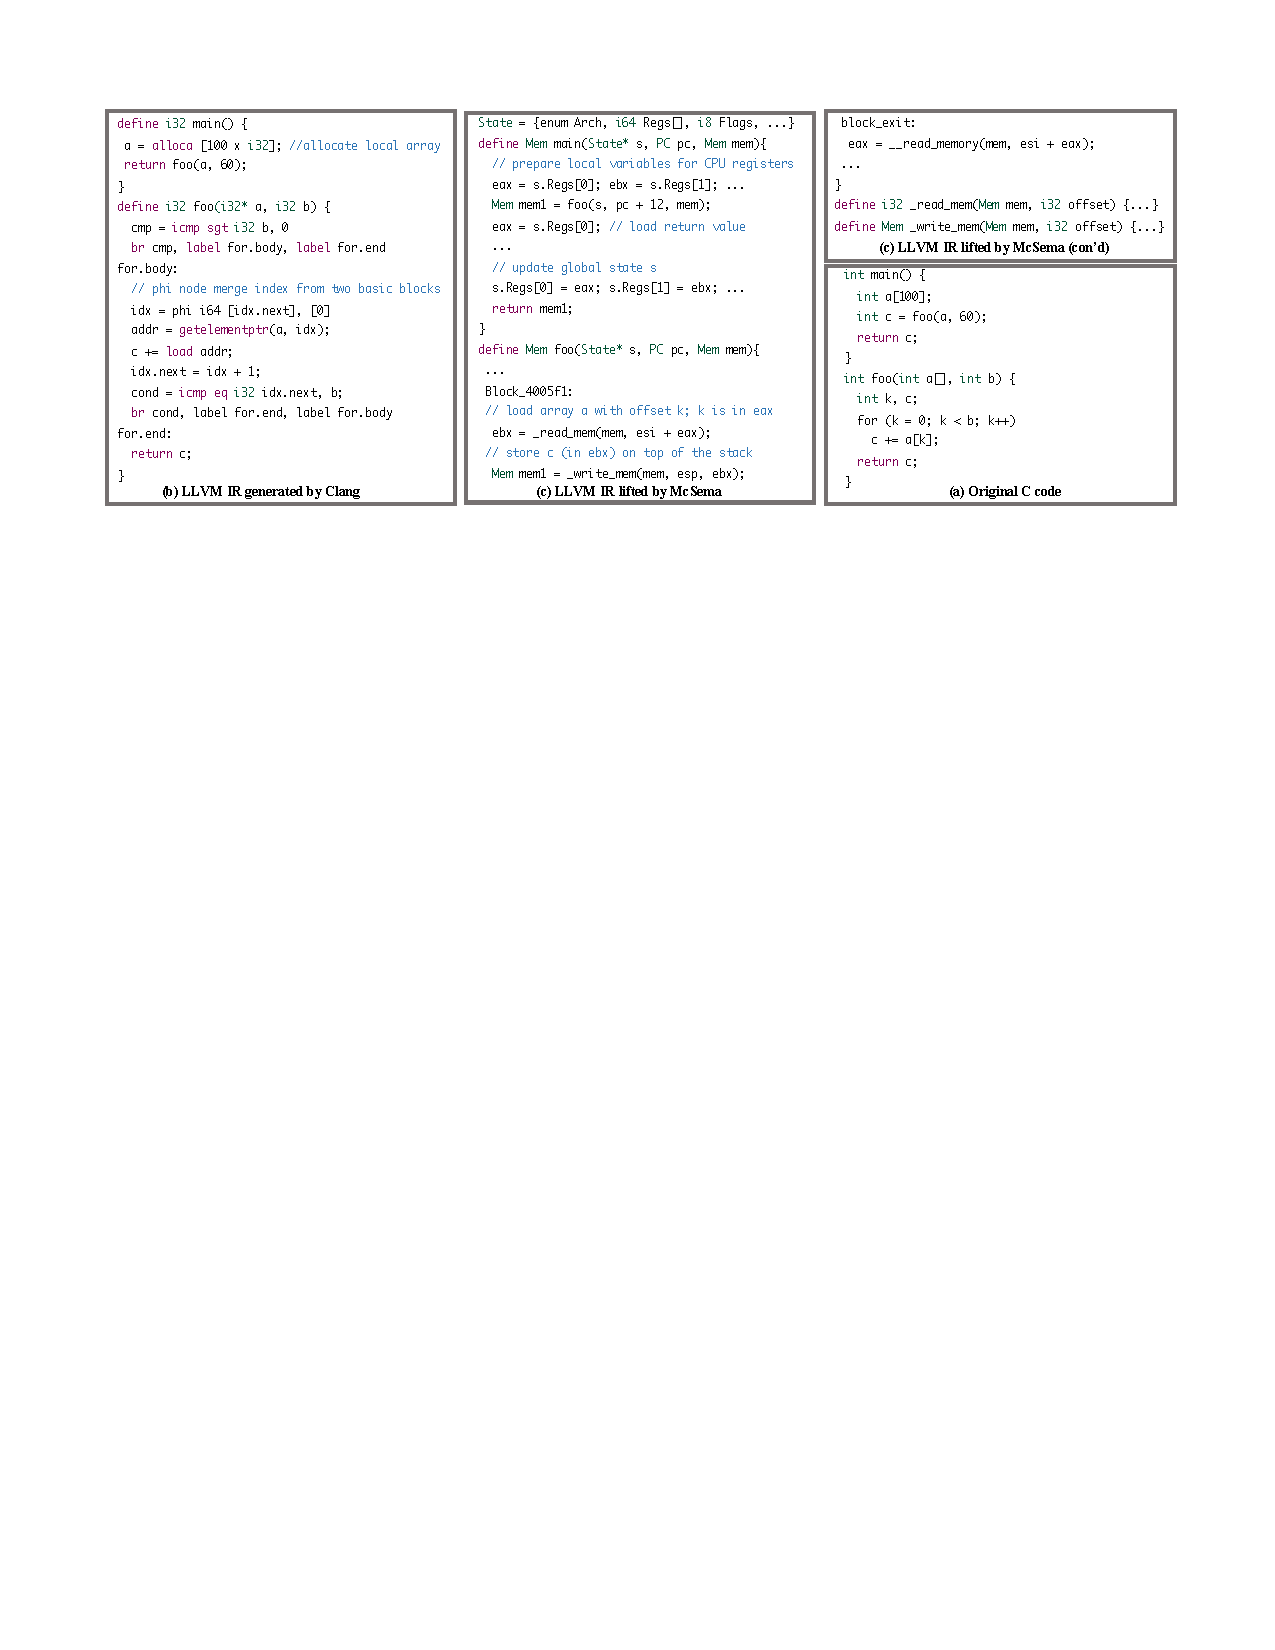
\includegraphics[width=1.0\textwidth]{fig/mcsema.pdf}
  \caption{A case study comparing LLVM IR lifted by McSema with LLVM IR compiled by Clang.}
  \label{fig:mcsema}
\end{figure}

As illustrated in \F~\ref{fig:mcsema}, IR lfited by McSema also does not contain variables, types, function signatures, and other higher-level information, which makes McSema lifted IR not a suitable target for transformation passes provided by the LLVM framework. The difference with BinRec is that McSema leverage the cutting-edge commercial reverse engineering tool, IDA~\cite{hex2014ida}, for static CFG recovery. Therefore McSema can statically transform and optimize the entire program without worrying about coverage.

On the other hand, Avast~\cite{avast} developed RetDec~\cite{retdec}, as a succinct-style lifter, tries to lift assembly to IR close to compiler-generated IR. However, as we discussed in \S~\ref{sec:challenges-variable}, recovering symbol or debugging information is unsolved. In most cases, RetDec cannot lift non-trivial programs into IR correctly and results in unfunctional rewritten binaries. Therefore, the output of RetDec is only used for tasks that do not require precise semantics, such as machine-learning-based program classification~\cite{ben2018neural} and manual inspection.


\subsection{Variables and Types Recovery} \label{sec:existing-recovery}
Although RetDec can hardly produce functional IR for non-trivial programs, it shows great potential in the program classification task. As shown in \F~\ref{fig:ncc}, we apply ncc (Neural Code Comprehension) method~\cite{ben2018neural} on five different lifter settings and compare the classification results with ncc based on compiler-generated IR. Mctoll~\cite{mctoll} is another \textit{succinct-style} lifter similar to RetDec, and McSema- represents McSema with all optimizations disabled. Lifters like RetDec and Mctoll show encouraging support for the classification task, whose performance is comparable to compiled IR.
Also, we find that lifters like RetDec have only implemented rudimentary analysis passes instead of advanced research products in the variables and types recovery field. So in this section, we will discuss recent variables recovery techniques that may further raise the upper bound of lifters.

\begin{figure}[tb]
  \centering
  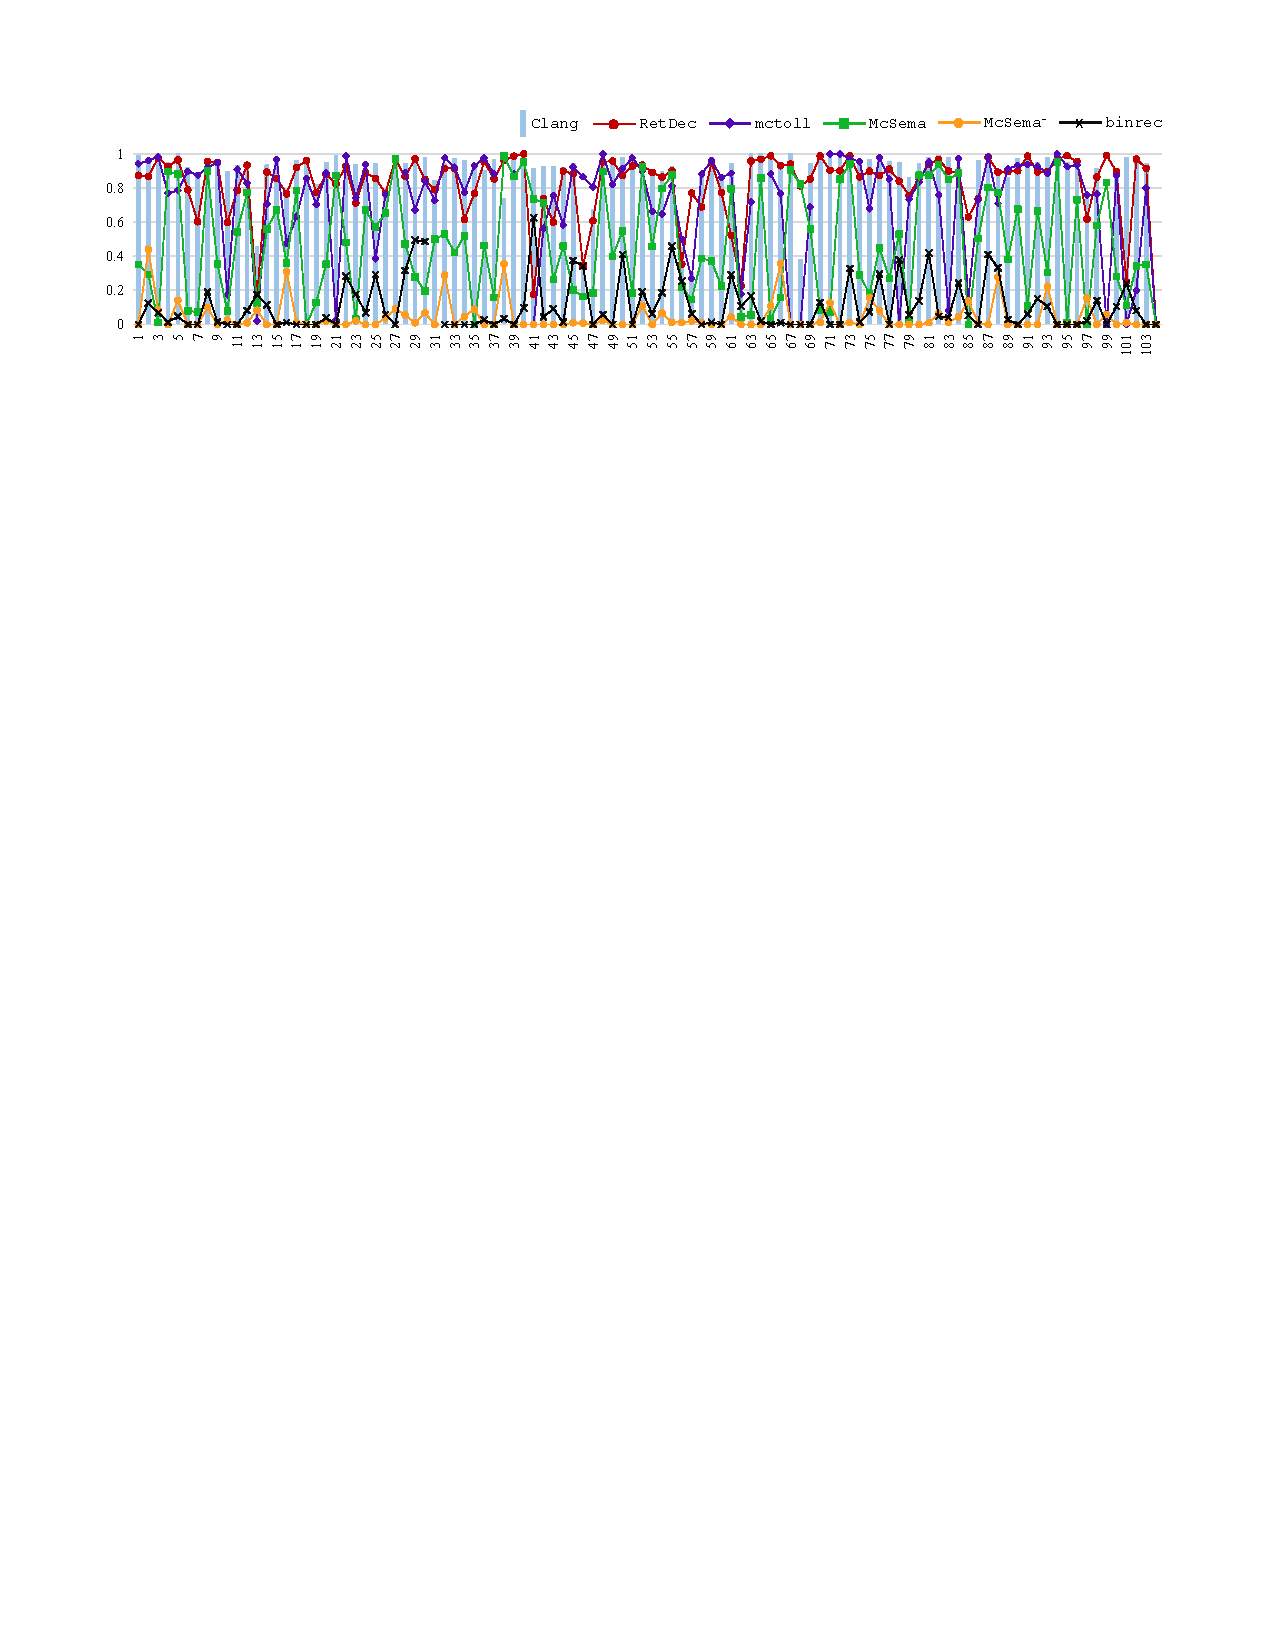
\includegraphics[width=1.0\textwidth]{fig/ncc.pdf}
  \caption{Classification analysis results of each tool across all 104 classes of the POJ-104 dataset.}
  \label{fig:ncc}
\end{figure}

\noindent\textbf{Dynamic Approaches.}~
% REWARDS
REWARDS uses a dynamic ``type sink'' technique to reveal program data structures from binaries automatically~\cite{lin2010automatic}. To be more specific, a timestamped attribute will be assigned to each memory location accessed. This attribute is propagated to other memory locations and registers during program execution. Once a type-revealing point or ``type sink'' that can resolve a variable's type is executed (e.g., the type revealing instructions, system calls, and library calls), the types of all memory locations sharing the same attribute are resolved. Similarly, another dynamic solution, Howard, aims to recover data structures from memory access patterns in execution traces~\cite{slowinska2011howard}. These dynamic approaches, while effective, are limited by coverage issues.

\noindent\textbf{Static Approaches.}~
% TIE
TIE proposes an end-to-end type inference system~\cite{lee2011tie}. It starts by lifting binary to BIL (BAP Intermediate Language) and finding variables with a variation of the VSA method named DVSA. The type system that consists of type inference rules is then used to generate constraints based on the BIL. Finally, the constraints are solved and lead to types as the results. TIE can produce accurate and conservative results, however, the heavyweight data flow analysis used for variable recovery makes it less practical in large binaries.
% SecondWrite
In the same way, SecondWrite~\cite{elwazeer2013scalable} makes a trade-off between accuracy and speed by combining a best-effort VSA variant for points-to analysis with a type-inference engine. Note that accurate types depend on high-quality points-to data, therefore less accurate points-to analysis will lead to a decrease in the accuracy of the results. Also, even original VSA is known to produce a lot of inaccurate results.
% Retypd
Comparably, Retypd (\textbf{re}gular \textbf{ty}pes using \textbf{p}ush\textbf{d}own) built on top of GrammaTech’s machine-code-
analysis tool CodeSurfer~\cite{balakrishnan2005codesurfer} introduces a principled static type-inference algorithm that supports more advanced types, including recursive types, polymorphism, and subtyping~\cite{noonan2016polymorphic}.

% Osprey
One of the latest probabilistic variables recovery techniques, \textsc{Osprey} (rec\underline{O}very of variable and data \underline{S}tructure by \underline{PR}obabilistic analysis for stripp\underline{E}d binar\underline{Y})~\cite{zhang2021osprey}, leverages a more advanced Path Sampling Driven Per-path Abstract Interpretation named BDA~\cite{zhang2019bda} instead of VSA for accurate and efficient points-to analysis. Moreover, as inevitable uncertainty in variable and structure recovery may result in contradicting predictions, \textsc{Osprey} introduces random variables in the type inference system to model the probabilities that a memory location is of a specific type. During type inference, probabilistic constraints are derived from these random variables and will be further solved to produce posterior probabilities as the recovery results. \F~\ref{fig:osprey} shows that \textsc{Osprey} achieves around 90\% precision, which substantially outperforms state-of-the-art commercial and open-source tools, including IDA~\cite{hex2014ida}, Ghidra~\cite{ghidra}, Angr~\cite{shoshitaishvili2016sok}, and Howard~\cite{slowinska2011howard}.

\begin{figure}[tb]
  \centering
  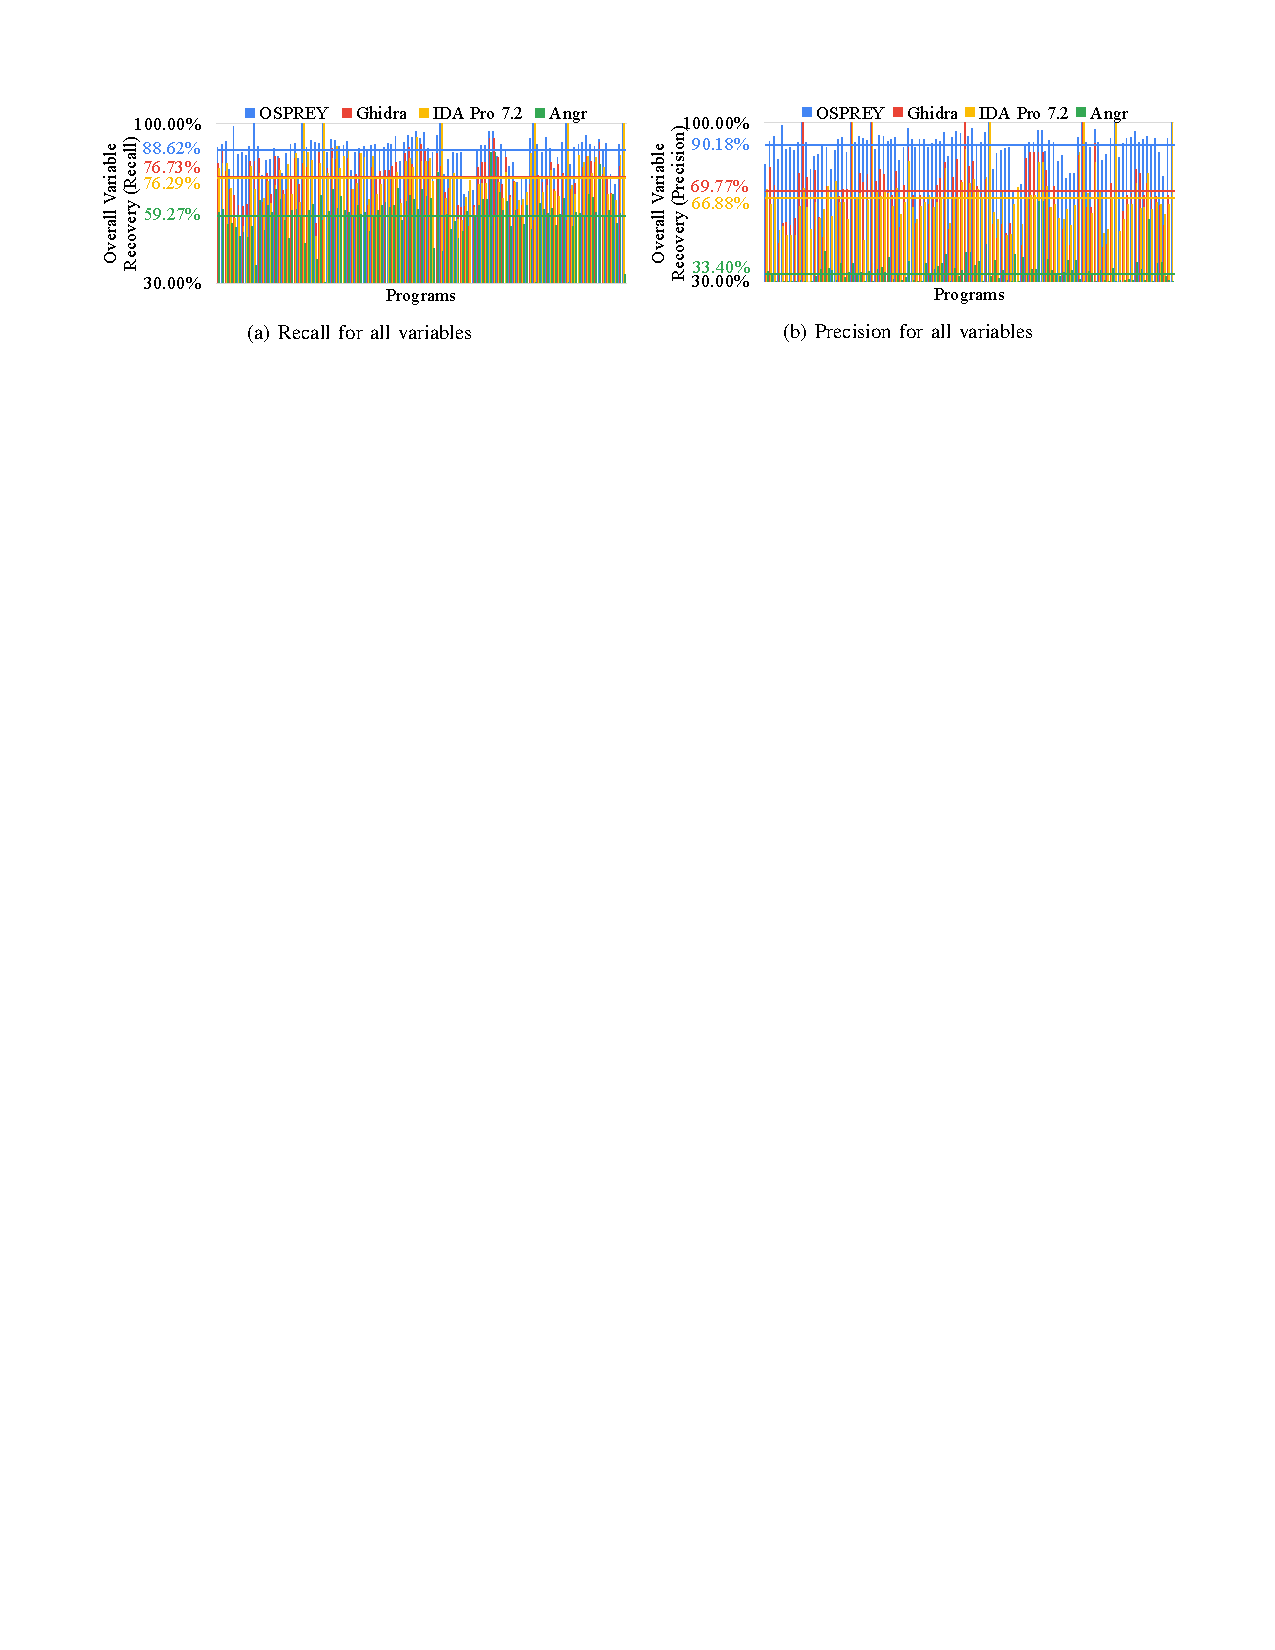
\includegraphics[width=1.0\textwidth]{fig/OSPREY.pdf}
  \caption{Presision and Recall of \textsc{Osprey}~\cite{zhang2021osprey}.}
  \label{fig:osprey}
\end{figure}

\noindent\textbf{ML-bassed Approaches.}~
% Debin
Machine learning has also been applied to recover variables and types. \textsc{Debin}~\cite{he2018debin} presents the first machine-learning-based approach to predict debugging information in stripped binaries. It combines an Extremely randomized Tree (ET)~\cite{geurts2006extremely} classification model with a linear probabilistic graphical model to recover properties of variables (e.g., symbol names, types, and locations). ET is used to extract unknown and known elements (variables) from lifted BAP-IR, then the linear probabilistic graphical model makes joint predictions on the debug information of elements. This approach effectively predicts symbol names and types with 68.8\% precision and 68.3\% recall on the x64 platform.
% CATI
CATI (Context-Assisted Type Inference)~\cite{chen2020cati} defines a new feature called Variable Usage Context (VUC) for type inference. The basic idea is based on the observation that neighboring instructions are likely to operate the same type of variables. Also, according to the empirical survey, only about 65\% of variables have more than 3 related instructions, which means 35\% of variables have only 1 or 2 related instructions. Thus to further improve the type inference accuracy, CATI first extracts the VUC feature that contains the target instruction with instruction context, then feeds the VUC feature into Word2Vec~\cite{mikolov2013distributed} model for assembly code embedding, finally, a multi-stage classifier with a convolutional neural network (CNN) is used to predict type for the target variable. The evaluation shows that CATI can achieve 71.2\% accuracy for type inference on unseen stripped binaries.


\subsection{Lifter Verification} \label{sec:existing-lifter-verfication}
Writing a precise binary lifter is extremely difficult even for those heavily tested projects, thus the verification of Lifter is an indispensable part of lifter-related research.
% MeanDiff ASE 2017
MeanDiff~\cite{kim2017testing} is the first lifter verifier that formally checks the semantic equivalence. It tested 3 binary lifters, including BAP~\cite{brumley2011bap}, PyVEX~\cite{pyvex}, and BINSEC~\cite{bardin2011bincoa}, by translating binary-based IRs (BBIRs) to a Unified Intermediate Representation (UIR) and generating symbolic summaries with data-flow analysis and symbolic execution. Although this method works on some low-level (does not contain variables information) IRs, it cannot be used to test LLVM IR lifters because it is more challenging to define a unified representation for lifted LLVM IR, in the sense that lifters aiming at different applications produce distinct results (i.e., emulation-style and succinct-style).

% PLDI 2020
Dasgupta et al.~\cite{dasgupta2020scalable} proposed a new lifter verification framework based on their previous work, in which they provided a complete formal semantics of x86-64 user-level instruction set architecture~\cite{dasgupta2019complete}. Their work is the first single-instruction translation validation framework using the formal semantics of x86-64 and IR. Similar to MeanDiff, it also uses symbolic execution to extract symbolic summaries from x86-64 and IR. With this framework, they proved that McSema is able to correctly translate 2254/2348 functions taken from LLVM's single-source benchmark test suite.
